%\part{Aspectos Metodológicos}

\chapter{Resultados Parciais}

Neste capítulo, serão apresentados alguns resultados que foram obtidos na primeira etapa da realização deste trabalho, que consistiu na revisão bibliográfica e estudo de trabalhos anteriores, no uso da linguagem Verilog e na realização de simulações mistas.

\section{Revisão Bibliográfica}

Na etapa inicial do trabalho, foi feita uma revisão bibliográfica sobre o tema, solidificando assim os conhecimentos sobre o cenário atual do uso da tecnologia RFID, tal como seu histórico e projeções futuras. Outra etapa importante para a realização do trabalho foi o levantamento de trabalhos anteriores no campo de RFID, mais especificamente sobre síntese de \textit{tags} passivas, que é o foco desde trabalho.

Como este projeto continua o trabalho realizado por outros alunos do curso de Engenharia Eletrônica na Faculdade do Gama, tais trabalhos são de extrema importância e relevância, em especial os trabalhos realizados no campo do \textit{front-end} analógico e do bloco digital, os dois grandes blocos que formam a \textit{tag}.

\section{Familiarização com a Linguagem Verilog e com as Ferramentas Utilizadas}

Foi realizado um estudo sobre a linguagem Verilog e sua estruturação, bem como sobre as ferramentas que serão utilizadas na realização deste trabalho, em específico, as ferramentas de simulação e síntese da \textit{Cadence}.

%\subsection{Verilog}

O Verilog é uma linguagem de descrição de \textit{Hardware} (do inglês, \textit{Hardware Description Language} - HDL) utilizada para descrever de forma textual a funcionalidade de sistemas e circuitos eletrônicos.
No escopo de projetos em Eletrônica, Verilog é utilizada para realizar verificações por simulação, análise temporal e síntese lógica, além de também ser utilizada para testes completos com avaliação de falhas e outras finalidades.

Outra característica importante do Verilog, é o fato dessa linguagem possuir diversos níveis de abstração, dos mais altos níveis com funções para modelagem de desempenho, até os mais baixos níveis de portas e chaves para verificação de projetos digitais e simulações comportamentais.

%A linguagem Verilog, juntamente com a linguagem VHDL, tem se tornado as duas principais linguagens utilizadas por projetistas de hardware tanto na indústria como no meio acadêmico.\cite{henriq}

%\subsubsection{Exemplos}

As figuras \ref{mux}, \ref{upcounter}, \ref{ff}, mostram alguns exemplos de módulos programados em verilog.

\begin{figure*}[ht!]
    \centering
    \begin{subfigure}[t]{0.5\textwidth}
        \centering
        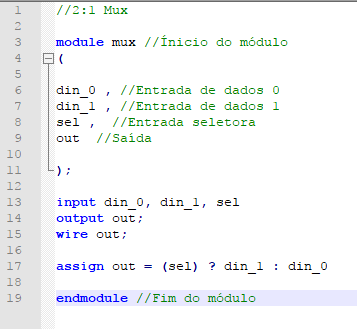
\includegraphics[height=2.5in]{figuras/mux.PNG}
        \caption{Módulo Mux}
        \label{mux}
    \end{subfigure}%
    ~ 
    \begin{subfigure}[t]{0.5\textwidth}
        \centering
        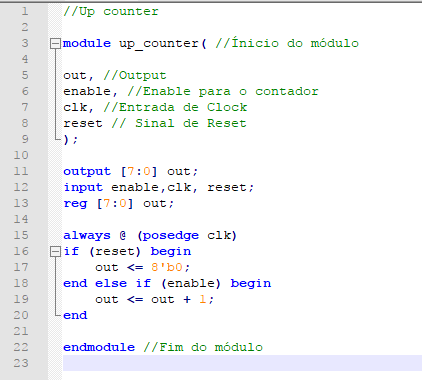
\includegraphics[height=2.5in]{figuras/upcounter.PNG}
        \caption{Módulo Contador}
        \label{upcounter}
        \end{subfigure}%
        
        ~ 
    \begin{subfigure}[t]{0.5\textwidth}
        \centering
        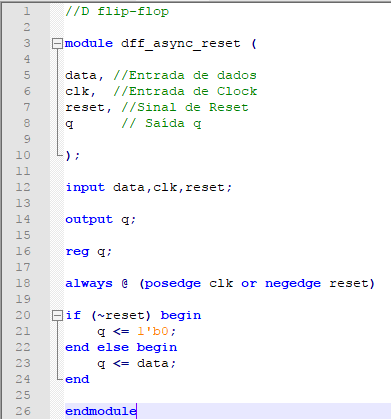
\includegraphics[height=2.5in]{figuras/ff.PNG}
        \caption{Módulo Flip-Flop}
        \label{ff}
    \end{subfigure}
    \caption{Exemplos de módulos em Verilog}
\end{figure*}

\section{Simulações Mistas}

As ferramentas da \textit{Cadence} permitem realizar a simulação de um sistema que possua tanto blocos analógicos como digitais para analisar se a comunicação entre eles está funcionando como o especificado. No caso do sistema de RFID, quando o leitor requer uma informação armazenada na memória da \textit{tag}, por exemplo, envia um sinal modulado para a mesma. O demodulador é o circuito responsável por recuperar a informação a partir do sinal modulado recebido.

Simulações realizadas em \cite{Marlon} demonstram que o bloco do demodulador funciona de forma satisfatória isoladamente. A modelagem em Verilog-AMS foi feita usando 3 sub-blocos: detector de envoltória, filtro de média e comparador com histerese. A Figura \ref{dem} mostra simulações do bloco demodulador realizadas em \cite{Marlon}, sendo possível observar as saídas intermediárias do detector de envoltória e do filtro de média.

\begin{figure}[ht!]
  \centering
  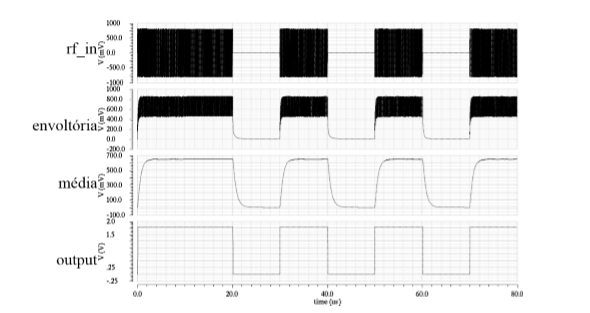
\includegraphics[width=\textwidth]{figuras/dem.PNG}
  \caption{Simulação do Demodulador ASK em Verilog-AMS\cite{Marlon}.}
  \label{dem}
\end{figure}

A simulação mista nos permite ver como este bloco se comporta quando conectado a um bloco digital. A Figura \ref{circ} mostra o teste do bloco modulador com um bloco simplificado de memória modelada em Verilog (\ref{memveri}). O intuito deste teste é apenas verificar a funcionalidade da interação entre blocos digitais e analógicos.

\begin{figure}[ht!]
  \centering
  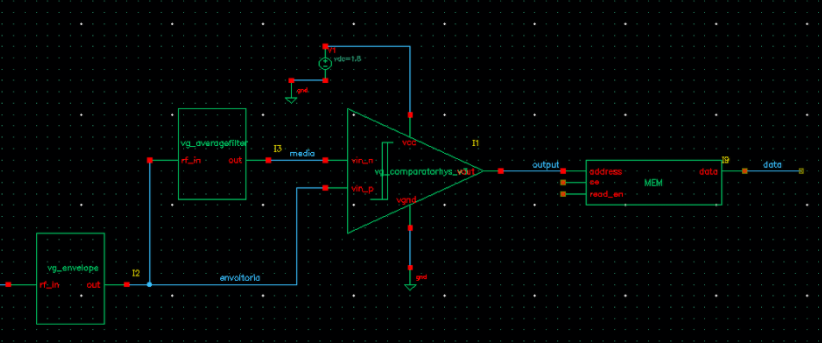
\includegraphics[width=\textwidth]{figuras/circ.PNG}
  \caption{Circuito com blocos analógicos e digitais.}
  \label{circ}
\end{figure}

\begin{figure}[ht!]
  \centering
  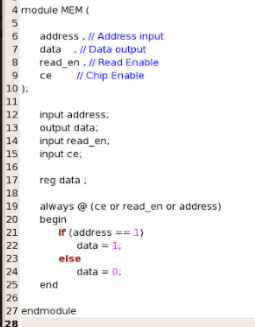
\includegraphics[width=0.5\textwidth]{figuras/mem.PNG}
  \caption{Modelagem do bloco digital de memória em Verilog.}
  \label{memveri}
\end{figure}

A Figura \ref{simdem} mostra o sinal de saída obtido com a simulação. Pode-se perceber que o bloco de memória responde corretamente ao sinal que vem do modulador, ou seja, o dado lido na memória é 0 para o endereço 0, e 1 para o endereço 1.

\begin{figure}[ht!]
  \centering
  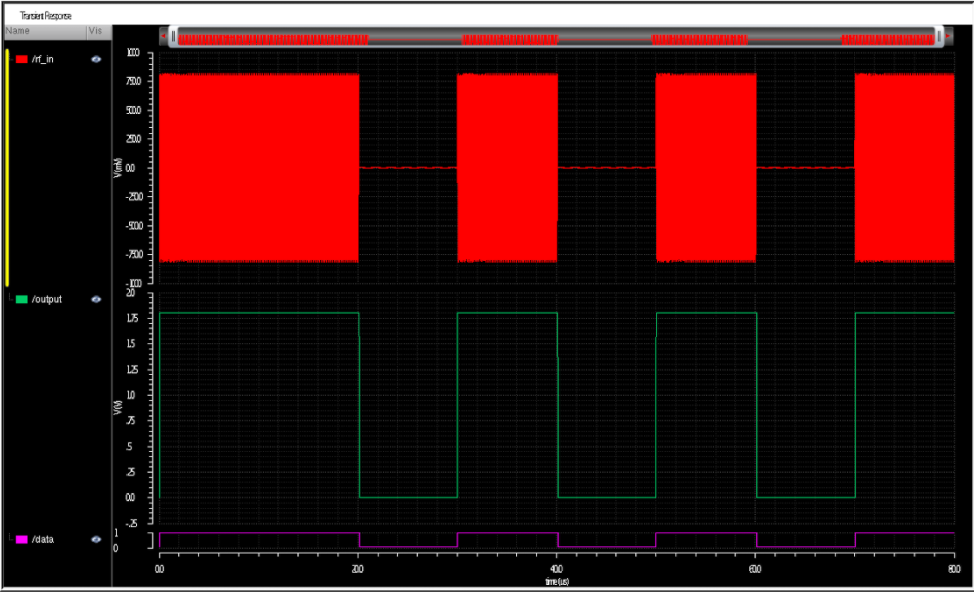
\includegraphics[width=\textwidth]{figuras/simdem.PNG}
  \caption{Resultado da simulação mista do demodulador e da memória.}
  \label{simdem}
\end{figure}

O próximo passo é simular o funcionamento deste conjunto com um bloco de memória mais complexo, com alguns bits de endereço e dados. Para tal, será necessário utilizar um bloco conversor serial-paralelo para se armazenar o valor do endereço enviado serialmente pelo demodulador.

% \section{Co-Simulação dos blocos analógicos com os blocos digitais}

